%%%%%%%%%%%%%%%%%%%%%%%%%%%%%%%%%%%%%%%%%%%%%%%%%%%%%%%%%%%%%%%%%%%%%%%%%%%%%%%%
% Implementation and algorithm details
%
%%%%%%%%%%%%%%%%%%%%%%%%%%%%%%%%%%%%%%%%%%%%%%%%%%%%%%%%%%%%%%%%%%%%%%%%%%%%%%%%


\chapter{Implementation}
In this chapter we discuss the design of the visualization system in brief. We
then look at some of the non-trivial issues that were encountered during the
implementation phase, what are their impact on the visualization as a whole and
our solutions.


%%%%%%%%%%%%%%%%%%%%%%%%%%%%%%%%%%%%%%%%%%%%%%%%%%%%%%%%%%%%%%%%%%%%%%%%%%%%%%%
\section{Environment and Architecture}
The implementation of this prototype is done in the Java programming language.
Graphics are rendered through Java for OpenGL graphics library. MySQL
database is used to host the raw text and document tags. Our graphics hardware
is a NVIDIA Quadro FX video card, and we were able to achieve a frame rate
between 15 to 30 FPS. The prototype is designed to run on 1680x1050 screen
resolution.

    % === Figure === 
	\begin{figure}
	 \centering  
	 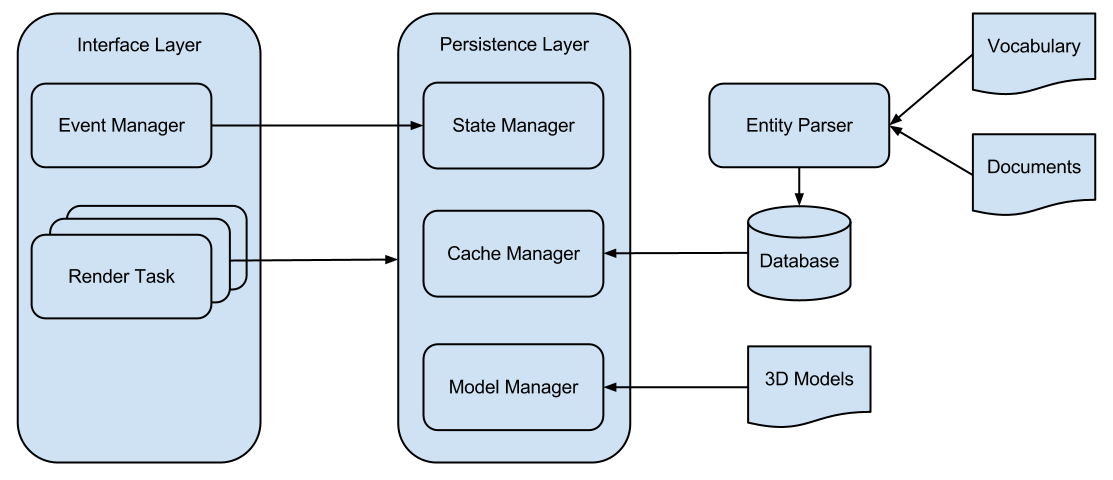
\includegraphics[width=\columnwidth]{Architecture.png}  
	 \caption{High level system architecture}
	 \label{figure:arch}
	\end{figure}
	% ==============

The application can be decomposed into two subsystems: a parser system for
generating entity scores and a visualization system. A  high level overview of
the system architecture is shown in Figure \ref{figure:arch}. The
entity parser consumes two inputs, the keyword hierarchy and the document texts, it
will then compute occurrence and co-occurrence scores and write the results to
the database, the parsing details are covered in Chapter 4. 
 
The visualization system implementation uses a standard two-tier design: A
persistence layer and an interface layer. The persistence layer is in charge of
database transactions, cached resources and system state. The interface layer takes
care of the rendering and any user triggered events. The visualization is
state-driven and the current state is stored in the persistent layer. The
primary reason for this is that this setup allows us to programmatically alter
the visualization independently of any other changes, and porting to other
platforms would likely only require changes to the Event Manager.

The major modules of our system, as well as their functionalities are listed below: 
\begin{itemize}[noitemsep]
  \item Render Task: Each rendering task is responsible for rendering a
  functional part of the interface. We have 4 primary rendering tasks: \threed
  visualization, filters, lens, and visual feedback. All rendering tasks poll
  the persistence layer at the beginning of their draw-loop to check if there
  are any updates.
  
  \item State Manager: State Manager keeps track of all states used to calculate
  the current visualization, as well as the states of all interactive elements.
  
  \item Model Manager: The model manager stores the \threed model geometries, it
  allows access to \threed information at various levels: models, components,
  polygons and finally vertices.
  
  \item Cache Manager: Cache Manager is responsible for handling all actions
  that impact the occurrence and co-occurrence scores, as well as any database
  queries.
  
  \item Event Manager: Event Manager listens to user interaction events, it
  communicate changes to the State Manager. All the hardware specific tunings
  reside in Event Manager.
\end{itemize}




%%%%%%%%%%%%%%%%%%%%%%%%%%%%%%%%%%%%%%%%%%%%%%%%%%%%%%%%%%%%%%%%%%%%%%%%%%%%%%%
\section{Algorithms}
During the development of the software prototype, we have encountered several
non-trivial problems. While these issues are not a part of our visualization 
design, they nonetheless impact the overall user experience via the degradation 
of aesthetic and usability of the system. In this section we discuss these 
problems and our proposed solutions.

\subsection{Order Independent Transparency}
Chapter 5 mentioned briefly that rendering translucent geometries in 3D space
can create artifacts, here we will describe this in greater detail and outline
our work around solution. There are two states that need to be toggeled to
enable translucent effetcs:
\begin{itemize} [noitemsep]
  \item Enable Blending: This option allows foreground objects to blend with
  background objects.
  \item Disable Depth Testing: This option renders all geometries regardless of
  depth and overlaps.
\end{itemize}

    % === Figure === 
	\begin{figure}
	 \centering  
	 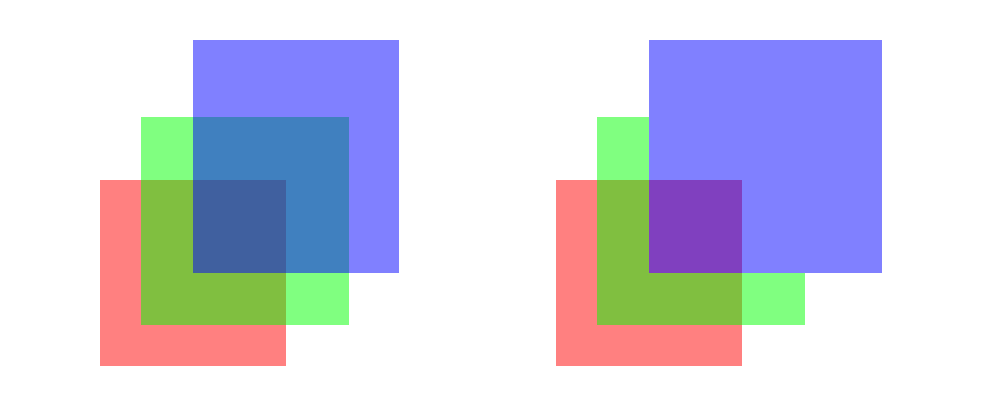
\includegraphics[width=\columnwidth]{oit_example.png} 
	 \caption[Order Independent Transparency]{The left image is rendered in
	 correct back-to-front order. The right image is out-of-order, the green
	 square does not properly blend into the blue square.}
	 \label{figure:oit}
	\end{figure}
    % =============

Geometries are typically not sent to the hardware in sorted order, so they are
neither front-to-back nor back-to-front. Hardware supported depth buffer
resolves the out-of-order polygons by selecting the fragment closest
to the viewing position. With transparent effect in place, fragments are blended
together rather than going through the selection process. Where the problem
arises is that alpha-blending is not commutative, for example: red+green+blue
is not equivalent to red+blue+green. The effects of out of order blending versus
in order blending is seen in Figure \ref{figure:oit}.

The major problem of out-of-order blending is that objects that are supposed to
be behind can appear to be in front, making it difficult for the viewers to
judge an object�s depth correctly. In the visualization, this is not only
distracting, but can mislead readers because it creates additional offsets
against the colouring scale.

Naively we can sort the geometries into depth order, or use space partitioning 
structures that forces the geometries to be depth order rendering. However, 
these naive solutions tend to have very expensive computation, and are view
dependent which results in re-computation whenever the viewing perspective
changes. There are also pathological cases where polygons intersect each other,
which cannot be solved with partitioning or sorting alone.

Alternative blending algorithm exist that looks at minimizing the effects of
order-dependent terms in blending equations, but there is a threshold on the
amount of transparency that can be applied~\cite{Meshkin2007, Bavoil2008}.
Other works use hardware features to allocate a buffer to emulate
sorting~\cite{Myers2007, Bavoil2008, Yang2010}, these algorithms produce more
accurate results, albeit bounded by hardware constraints or the complexity of
the scene itself.  

In this prototype, we use an implementation of dual-depth-peeling
\cite{Bavoil2008}, which ``peels'' the \threed scene apart layer by layer
into textures, before recomposing these texture into a final texture in depth order. The implication 
of this peeling effect is that it effectively changes the rendering process from
single to multiple passes, a complete rendering will take N/2 passes where N is
the number of geometric layers based on the present viewing position. This 
method yield accurate and eye-pleasing results, while more performance friendly
methods exists, we decided that this was the most reasonable approach because
the required features are available on most hardware at the time of implementation.
  


% \subsection{Effects}
% Here we briefly discuss our usage of graphical effects. OIT rendering, as
% described above, is used to ensure correct depth cues, it is possible to achieve
% different look and feel by passing different lighting equations to the shader
% programs. Halo effect is done by calculating silhouettes in \twod space of the
% active entities, we then subtract the geometric shape from the silhouette, and
% perform a smoothing step to blur out sharp features on the outline. The ghostly
% outline effect is done by calculating ridge and silhouette edges of adjacency
% structures in the mesh, as outlined in Hermosilla's GPU implementation
% \cite{Hermosilla2009}. Finally the lens effect is achieved through adding and
% subtracting of textures, the full scenes with lens semantic is rendering into a
% texture, we alter the non-lens area to be completely transparent and superimpose
% the remainder onto the existing scene.

 

\subsection{Cache and Stabilization}
Because the size of the dataset used to render the visualization can vary
greatly, database query performance tends to vary as well. To compound the
problem, most queries in the system are aggregation based queries and create
additional performance overhead. Overall database execution time can vary from a
few milliseconds to several seconds, we found this to be unacceptable because
it degrades user experiences.

Here we introduce an intermediate in-memory cache to store the aggregated scores
of each entity. The cache is initialized once at system initialization,
afterwards queries are executed against the cache  rather than the database.
The cache organization is specific to this dataset, however the idea itself is
generalizable.

Cache is realized as a hierarchy of lookup tables. It is modelled based on
the time and hierarchy filters and how we perceive people use the visualization.
The cache levels are, from most general to most specific: time period, entity,
manufacturer, make, model and model year. 

Each node in the cache hierarchy contains three things, a reference to all its
direct children, an aggregated score of all its children, and a reference to the
documents that matches the node which are used to calculate co-occurrence. For
example, a node corresponding to (July 2010, engine) will have the following:
\begin{itemize}[noitemsep]
  \item An aggregated score total that indicate the number of occurrence of
  engine in documents relating to incidents during July 2010
  
  \item A listing of unique document IDs that matches the above criteria
  
  \item References to children nodes (manufacturers) that matches the above criteria
\end{itemize}

The overview visualization is then constructed by iterating over the desired
time periods, apply the hierarchy filter to find the correct cache node for each
entity, and then sum up the node's entity score across the time periods. Because
the aggregations are done ahead of time at system start up, and because score
lookup is constant time, our cache results in an a much more stable performance
compared against database queries. On average we found the cache queries take
about 100 to 200 milliseconds to complete, which we found to be acceptable.




%Due to the size of our data and the diverse variations of queries on the
% database, we have encountered situations where our database does not produce a stable 
%performance. We have found with SQL queries alone our query results come back 
%between several milliseconds to a few seconds. A major part of this delay is due 
%to the nature of the queries, which are mostly aggregates that result in sorting 
%operations. We found this to be unacceptable, because it defies people�s 
%expectation of instantaneous reaction from the system.

% To create a better user experience in-line with user expectations, we created
% a hierarchical lookup table that partially caches the aggregated query results. 
% Each level corresponds to a unique filtering criteria based on our dataset, for 
% this prototype, we have from highest level to lowest level : time, entity, 
% manufacturer, make, model and year. The hierarchy order models the type of 
% successive query refinement we expect of typical interactions. Each entry, in any 
% level, corresponds to the aggregated query up to that specific point. Each entry 
% contains a value that is the aggregated count of the documents, as well as a 
% reference to a list of its children, if applicable. For example: (``2000'',
% ``engine'', ``Toyota'') will yield the query results of all Toyota vehicle
% complaints that had engine problems in the year 2000. To create ranged query, for example 2000 to 2005, we 
% issue the same query with different time parameters and sum up the results. More 
% complex queries such as aggregation and co-occurrences, are done in similar manner, 
% but with different lookup tables. In practice, we found this to be a middle of the 
% road approach. Comparing to raw database queries, it performs slower than best case 
% but much faster than the worst case scenarios, most important of all, we have 
% consistent performance at around 100 to 200 millisecond, which we found to be 
% acceptable for interactive use.
% 
% The table is created at when system starts, we iterate through the database
% tables once, creating the hierarchy structure and increment the counts as we go. As a last 
% optimization step, we have attempted to serialize out the query tables to disk, 
% so they can be de-serialized on system startup without having to iterate the
% database tables. However, without a customized data container, this in practice turned out 
% to be slower than database lookups and was abandoned.


\subsection{Multi-Touch Heuristics}
Touch sensors have a few drawbacks, there are inherent noises that come from
performing gestures, in addition, our inability to hold our hands perfectly
still accentuate this issue by creating jitters. In our particular use case, the
upright display makes certain gestures difficult, for example, in an informal
evaluation of the display we found that certain curvatures introduced noises
because the knuckles of other fingers are sensed as false-positive touch points
as a result of drifting too close to the screen itself.

These noises degrades user experiences, as they trigger unexpected events within
the system. We introduce a set of software heuristics as an intermediate step
between when the points are sensed and when they are executed. In general, these
heuristics remove unintended touches and prevent jittery animations that
result from minute movements. While these are designed specifically to deal with
our hardware issues, we believe rules are general enough that they can be
adopted to other touch sensors. 

\begin{itemize} [noitemsep]
  \item \textbf{Real Update:} The muscle deformation when pressed against the
  display, paired with inability to keep perfect still postures result in
  sensor registering jittery updates. This is undesirable because it induces a
  shaking effect, and often time unnecessary because the updates are minute.
  To compensate this problem, the system only accept an update if it is at least
  X number of pixels away from the previous updated point.
  
  \item \textbf{Coincidental Points:} When a touch is initialized on the touch
  surface, there is a possibility that more than one touch point will be
  registered. This is similar to the case we presented above. To reduce this scenario from
  occurring, we store the XY-coordinate and the time that the touch point is
  created. If a touch point is created too close to any other touch point within a time
  threshold X, that point is rejected.
  
  \item \textbf{Movement Buffer:} When a gesture is in transition, there are
  cases where other parts of the hand will inadvertently cause false-positives.
  We try to neutralize these occurrences by introducing buffer zones around touch
  points that are in transition. New touch points cannot be created 
  if they fall within X pixels away from a point that is in transition.
  
  \item \textbf{Reinforce Intention:} This heuristic deals with reducing jitters
  on the initial touch. This can be seen as a special case of the Real Update
  heuristic, but while Real Update toss away extremely small update in general,
  the first update can be quite large, probably due to the act of pressing the
  finger against the display. We made it such that the first update must be at
  least X pixels distance in magnitude. This heuristic is not applicable to
  lens widget nor document widget because we want them to be immediately
  responsive. 
  
  \item \textbf{Dead Zones:} In some cases, the act of lifting up
  a finger to disengage a gesture will trigger a new touch point. This makes
  selection problematic, as selected entities will be deselected right away. To
  resolve this issue the system impose dead zones. When a touch is removed, the
  area around it will become unavailable for a small amount of time, during
  which all new touch points are ignored.
  
\end{itemize}


